\documentclass[12pt,pdftex,a4paper]{article}
\usepackage[ngerman]{babel}
\usepackage[utf8]{inputenc}
\usepackage{amsmath}
\usepackage{amssymb}
\usepackage{ulem}
\usepackage{bbm}
\usepackage{array}
\usepackage{marvosym}
\usepackage{color}
\usepackage{hhline}
\usepackage[pdftex]{graphicx}
\usepackage{listings}
\lstset{language=Python,basicstyle=\footnotesize}
\usepackage{pdfpages}
\usepackage{booktabs}
\PassOptionsToPackage{hyphens}{url}
\usepackage{hyperref}
\usepackage{extarrows}
\usepackage{rotating}
\usepackage{dsfont}
\usepackage{circuitikz}
\newcommand\tab[1][1cm]{\hspace*{#1}}

\usepackage{eurosym}
\def\bitcoinA{%
  \leavevmode
  \vtop{\offinterlineskip %\bfseries
    \setbox0=\hbox{B}%
    \setbox2=\hbox to\wd0{\hfil\hskip-.03em
    \vrule height .3ex width .15ex\hskip .08em
    \vrule height .3ex width .15ex\hfil}
    \vbox{\copy2\box0}\box2}}

\usepackage{fancyhdr}
\pagestyle{fancy}
\lhead{Franziska Hutter(3295896) - 
	Felix Truger(3331705) - 
	Felix Bühler(2973410)}
\renewcommand{\headrulewidth}{0.6pt}

\title{Security and Privacy,\\ Blatt 5}
\author{Franziska Hutter (3295896)\\
	Felix Truger (3331705)\\
	Felix Bühler (2973410)}


\begin{document}
\maketitle
\pagebreak

\section*{Problem 1: Schnorr’s protocol - special honest verifier zero-knowledge}

% SEE for reference: http://www.cs.au.dk/~ivan/Sigma.pdf
% https://cs.nyu.edu/courses/spring07/G22.3220-001/lec2.pdf
% danieleventuri.altervista.org/files/zero-knowledge.pdf (contains proof)

It is easy to see, that $(P, V)$ as given for Schnorr’s protocol has the form of a $\Sigma$-protocol with commitment $a$, challenge $e$ and response $z$.
The ``special honest verifier ZK'' property requires: $\exists$ ppt simulator $M$ such that $\forall x\in L_R$ and $e\in \{0,1\}^t: M(x, e) = Trans_{V^e}^P(x)$ where $Trans_{V^e}^P(x)$ is the Transcript of an interaction between (honest) $P$ and $V$ using challenge $e$ on input $x$ and equality refers to an identical distribution.
\\~\\
$M$ works as follows:
\begin{itemize}
\item Receive inputs $(\mathcal{G},q,g,h)$ and $e$.
\item Select $z\in\mathbb{Z}_q$ randomly.
\item Calculate $a = \frac{g^z}{h^e}\mod q$.
\item Output transcript $(a, e, z)$.
\end{itemize}\
\\
On the calculation of $a$:\\
We know from the protocol, that $P$ calculates $z$ as follows:
$$z=r+e\cdot w \mod q$$
Since $\mathcal{G}$ is cyclic with generator $g$:
$$g^z = g^{r+e\cdot w \mod q} = g^r \cdot g^{e\cdot w \mod q}$$
We also know:
$$g^r = a; g^w=h$$
$$\implies g^z = a \cdot h^e \mod q$$
Thus a valid $a$ can be calculated as follows:
$$a = \frac{g^z}{h^e} \mod q$$
\\
As for the probability distribution of a transcript of $(P,V^e)$, we know that $r\in \mathbb{Z}_q$ is selected randomly by the honest prover and thus $a = g^r$ is indirectly selected randomly as well with the same distribution as for $r$. Note again, that $\mathcal{G}$ is cyclic. $z$ on the other hand directly depends on the other values and can be calculated by a deterministic function, as it is actually performed by $P$.\\
We have the same probability distribution for $M$, as $z\in \mathbb{Z}_q$ is selected at random. $a$ is then deterministically calculated from $e$ and $z$. Just the other way around.\\
More precisely we have the same probability space $(\Omega, 2^{\Omega}, P)$ in both cases, where
\begin{itemize}
\item $\Omega = \mathbb{Z}_q$
\item $P: 2^{\Omega} \rightarrow [0,1]$ is a uniform distribution.
\end{itemize}\
It follows from the above, that Schnorr's protocol fulfills the ``special honest verifier ZK'' property.

\section*{Problem 2: Homomorphic properties of algorithms}
$p=(\mathcal{G},q,g,h)$ fixed, $r_0, r_1, v_0, v_1 \in \mathbb{Z}_q$, we show:
$$com^{r_0+r_1}(p, v_0 + v_1) \overset{!}{=} com^{r_0}(p, v_0) \cdot com^{r_1}(p, v_1)$$
By just applying the definition of $com$ in the Pedersen commitment scheme, we know:
$$com^{r_0+r_1}(p, v_0 + v_1) = g^{v_0 + v_1}\cdot h^{r_0+r_1}$$
$$com^{r_0}(p, v_0) = g^{v_0} \cdot h^{r_0}$$
$$com^{r_1}(p, v_1) = g^{v_1} \cdot h^{r_1}$$
Thus:
$$com^{r_0}(p, v_0) \cdot com^{r_1}(p, v_1) = g^{v_0} \cdot h^{r_0} \cdot g^{v_1} \cdot h^{r_1}$$
$$= g^{v_0}\cdot g^{v_1}\cdot h^{r_0}\cdot h^{r_1}$$
$$= g^{v_0 + v_1}\cdot h^{r_0+r_1}$$
$$= com^{r_0+r_1}(p, v_0 + v_1)$$

% This definitely seems TOO EASY?!?

\section*{Problem 3: Building circuits for functions}
Find the drawing of our circuit for $f$ below.\\
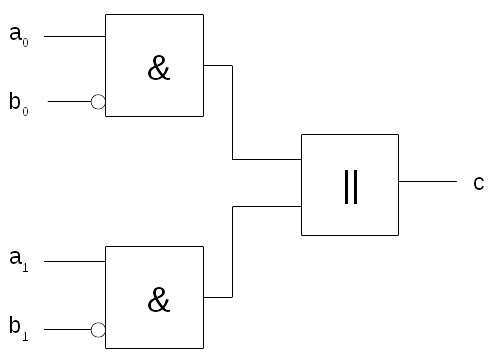
\includegraphics[width=200pt]{./problem3_binary_circuit.png}

\section*{Problem 4: Garbled circuits}
Find a garbled circuit for the given circuit below.\\
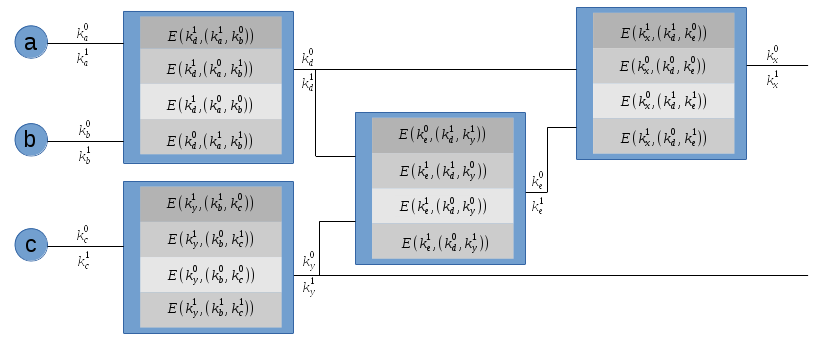
\includegraphics[width=475pt]{./problem4_garbled_circuit.png}
Note that we simplified the circuit by replacing the AND gate in the middle by a NAND gate, so we do not need an additional NOT gate to get the inverse of the input for the following XOR gate.

\section*{Problem 5: 51\%-Attack on Bitcoin}
\subsection*{(a)}
With 49\% of the hash-power a block is found within 20 minutes on average, i.e. 3 blocks per hour. Thus 51\% of the hash-power can find $\frac{3}{49\%}\cdot 51\% \approx 3.12245$ blocks per hour. The attacker needs to find 6 blocks more than the honest part of the network in the same time. This is: $t\cdot 0.12245 = 6$, which leads to $t \approx 49$ hours needed to catch up with the honest branch.
\subsection*{(b)}
In the calculated 49 hours the attacker generates $3.12245 \cdot 49 \approx 153$ new blocks. Obviously the difference between the earnings and costs for finding a block is $100,000\frac{\text{\euro}}{block} - 12.5\frac{\bitcoinA}{block}\cdot 6,000\frac{\text{\euro}}{\bitcoinA} = 25,000\frac{\text{\euro}}{block}$. Thus the attacker would need to make an additional $25,000\frac{\text{\euro}}{block} \cdot 153 blocks = 3,825,000\text{\euro}$ via double-spending to compensate his costs. Under the given circumstances $3,825,000$\EUR{} were worth approximately $637.5$\bitcoinA. To make a profit, the attacker would need to double-spend at least a bit more than the aforementioned amount.
\subsection*{(c)}
Ideas to make a 51\% attack more efficient:
\begin{itemize}
\item The attacker could simultaneously to his attack manipulate the network such that newly found blocks are not communicated properly to all parties. The propagation of blocks relies on the gossip protocol. If the attacker prevents the proper communication between parties, different mining pools might work on different versions of the blockchain (i.e. one pool does not know that a new block is already found and keeps working on an old version of the chain), thus the hash-power of the honest miners may be splitted, leading to an advantage for the attacker.
\item Similarly the attacker might even be able to manipulate mining pools to work on his own branch of the blockchain, by propagating it as the latest version and hindering the propagation of the honest branch to certain mining pools. (Note: This method requires the attacker to separate the network ideally beforehand or alternatively once his blockchain is close to the honest blockchain.)
\end{itemize}

\end{document}